\documentclass[conference]{IEEEtran}

% ---- Packages ----
\usepackage[utf8]{inputenc}
\usepackage[T1]{fontenc}
\usepackage{amsmath,amssymb,amsthm}
\usepackage{algorithmic}
\usepackage{algorithm}
\usepackage{booktabs}
\usepackage{multirow}
\usepackage{graphicx}
\usepackage{tikz}
\usetikzlibrary{matrix,positioning,fit,backgrounds,calc}
\usepackage{pgfplots}
\pgfplotsset{compat=1.18}
\usepackage{listings}
\usepackage{xcolor}
\usepackage{balance}
\usepackage{url}
\usepackage{cite}
\usepackage{hyperref}
\hypersetup{hidelinks}

% ---- Theorem environments ----
\newtheorem{theorem}{Theorem}
\newtheorem{property}{Property}
\newtheorem{definition}{Definition}

% ---- Listings style for SQL ----
\lstdefinestyle{sql}{
  language=SQL,
  basicstyle=\ttfamily\scriptsize,
  keywordstyle=\bfseries\color{blue!70!black},
  commentstyle=\itshape\color{green!50!black},
  stringstyle=\color{red!60!black},
  showstringspaces=false,
  breaklines=true,
  frame=single,
  framesep=2pt,
  xleftmargin=4pt,
  xrightmargin=4pt,
  aboveskip=6pt,
  belowskip=4pt,
  morekeywords={RETURNS,TABLE,RETURN,FUNCTION,NVARCHAR,DATETIME2,LTRIM,RTRIM,CREATE,WITH,UNION,ALL,SELECT,FROM,WHERE,INNER,JOIN,ON,AS,IN,TOP,AND,OR,IS,NULL,INT,MAX}
}

% ---- Pseudocode style ----
\lstdefinestyle{pseudo}{
  basicstyle=\ttfamily\scriptsize,
  keywordstyle=\bfseries,
  showstringspaces=false,
  breaklines=true,
  frame=single,
  framesep=2pt,
  xleftmargin=4pt,
  xrightmargin=4pt,
  aboveskip=6pt,
  belowskip=4pt,
  morekeywords={ALGORITHM,FOR,EACH,IN,IF,RETURN,WHERE,EXISTS}
}

% ---- C# style ----
\lstdefinestyle{csharp}{
  language=[Sharp]C,
  basicstyle=\ttfamily\scriptsize,
  keywordstyle=\bfseries\color{blue!70!black},
  commentstyle=\itshape\color{green!50!black},
  stringstyle=\color{red!60!black},
  showstringspaces=false,
  breaklines=true,
  frame=single,
  framesep=2pt,
  xleftmargin=4pt,
  xrightmargin=4pt,
  aboveskip=6pt,
  belowskip=4pt,
  morekeywords={var,async,await,string,IQueryable,Expression,Func,Task,bool,where},
  literate={=>}{{\textcolor{blue!70!black}{=>}}}{2}
}


\begin{document}

% ---- Title ----
\title{Database-Native Authorization for Human and Autonomous Principals: The SHRBAC Model}

% ---- Double-blind: anonymous authors ----
\author{\IEEEauthorblockN{Anonymous Author(s)}
\IEEEauthorblockA{Removed for double-blind review}}

\maketitle

% ===========================================================================
% ABSTRACT
% ===========================================================================
\begin{abstract}
Enterprise applications must answer two authorization questions: ``can this principal act on this resource?'' (point check) and ``which resources can this principal access, filtered, sorted, and paginated?'' (list filtering). Point checks are boolean decisions with well-understood evaluation strategies. List filtering is fundamentally harder: it requires composing authorization decisions with application-defined filtering, sorting, and pagination into a single efficient query---and when authorization logic resides outside the database, an impedance mismatch arises. We present SHRBAC (Scoped Hierarchical Role-Based Access Control), a formal authorization model whose structural constraints---tree-structured resources, flat roles, polymorphic principals including autonomous agents---guarantee that enforcement is a composable database predicate with bounded cost---concretely, a parameterized inline Table-Valued Function (TVF) that the optimizer folds into the execution plan. The model enforces the principle of least privilege through grants scoped by resource subtree, role, and time window, enabling both human users and AI agents to operate with minimum necessary authority. We formalize the model, prove soundness and completeness of the TVF enforcement, and show that under cursor pagination, per-page cost is $O(k \cdot D)$---predictable, linear, and independent of total dataset size. Empirical evaluation on SQL Server 2022 with 1.2M resource nodes ($D{=}5$) and 1.5M resource nodes ($D{=}10$) confirms $N$-independence across three orders of magnitude.
\end{abstract}

\begin{IEEEkeywords}
access control, RBAC, authorization, query composition, table-valued function, resource hierarchy, agentic AI
\end{IEEEkeywords}

% ===========================================================================
% 1. INTRODUCTION
% ===========================================================================
\section{Introduction}

\subsection{The Problem}

Modern B2B SaaS applications require authorization systems that answer two fundamentally different questions:

\begin{enumerate}
\item \textbf{Point check}: ``Can principal $p$ perform action $a$ on resource $r$?''---a boolean decision.
\item \textbf{List filtering}: ``What resources of type $T$ can principal $p$ access, given search criteria $C$, sorted by $S$, paginated to page $k$?''---a set-returning query integrated with application data.
\end{enumerate}

The first question is well-understood. Google's Zanzibar~\cite{zanzibar} and its descendants handle millions of point checks per second through graph traversal and caching.

The second question---the \textbf{list filtering problem}---is well-solved for flat access models. A single-tenant predicate (\texttt{WHERE tenant\_id = @currentTenant}) composes trivially. However, when access is determined by grants at varying levels of a resource hierarchy, resolved through transitive group memberships, and subject to temporal constraints, list filtering becomes substantially more complex.

Increasingly, principals are not only human users but \textbf{autonomous AI agents} that issue queries and perform actions over enterprise data. These agents operate in loops, enumerating and filtering large resource sets programmatically. For agentic systems, efficient list filtering is not merely a user-experience optimization---it is a correctness and cost requirement. An agent that makes $N$ external authorization calls per page degrades linearly; an agent whose authorization is a composable database predicate operates at constant cost per page.

Beyond efficient querying, the authorization model must enforce the \textbf{principle of least privilege}~\cite{saltzer}: principals, whether human or autonomous, should operate with minimum necessary authority scoped to specific resources and time windows. For AI agents, this is not merely good practice but a safety requirement---an agent should receive a narrow grant (specific subtree, limited role, bounded duration) rather than broad access.

When authorization logic resides outside the database, an impedance mismatch arises. Industry bridges this gap through ID lookups, batch post-filtering, partial policy evaluation, or materialized permission views---each trading scalability, consistency, or complexity. Some of these approaches are SQL-implementable, but they require runtime predicate construction that changes shape as the policy set evolves.

SHRBAC takes a different approach: the model's structural constraints are chosen so that per-page enforcement cost is $O(k \cdot D)$---linear in page size and tree depth, independent of total resource count $N$ and policy set size (Fig.~\ref{fig:enforcement}).

% ---- FIGURE: Enforcement artifact vs policy count ----
\begin{figure}[t]
\centering
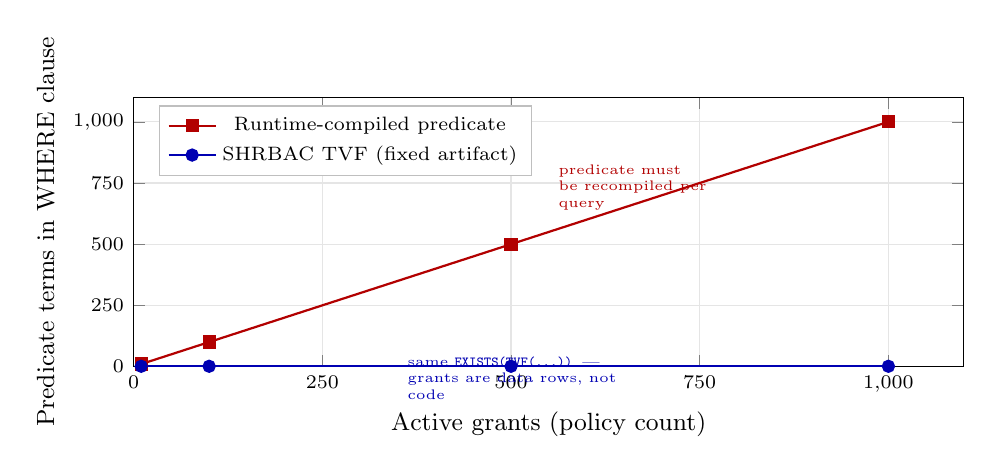
\begin{tikzpicture}
\begin{axis}[
    width=\columnwidth,
    height=5.0cm,
    xlabel={Active grants (policy count)},
    ylabel={Predicate terms in WHERE clause},
    xmin=0, xmax=1100,
    ymin=0, ymax=1100,
    xtick={0,250,500,750,1000},
    ytick={0,250,500,750,1000},
    legend style={at={(0.03,0.97)}, anchor=north west, font=\scriptsize, draw=gray!50},
    grid=major,
    grid style={gray!20},
    every axis label/.style={font=\small},
    every tick label/.style={font=\scriptsize},
    clip=false,
]

% Runtime-compiled: predicate grows linearly with grants
\addplot[
    color=red!70!black,
    thick,
    mark=square*,
    mark size=2pt,
    mark repeat=1,
] coordinates {
    (10, 10)
    (100, 100)
    (500, 500)
    (1000, 1000)
};
\addlegendentry{Runtime-compiled predicate}

% SHRBAC: constant — always 1 TVF invocation
\addplot[
    color=blue!70!black,
    thick,
    mark=*,
    mark size=2pt,
    mark repeat=1,
] coordinates {
    (10, 1)
    (100, 1)
    (500, 1)
    (1000, 1)
};
\addlegendentry{SHRBAC TVF (fixed artifact)}

% Annotation on the growing line
\node[font=\tiny, text=red!70!black, anchor=south west, text width=2.2cm] at (axis cs:550,600) {predicate must be recompiled per query};

% Annotation on the flat line
\node[font=\tiny, text=blue!70!black, anchor=north west, text width=2.8cm] at (axis cs:350,80) {same \texttt{EXISTS(TVF(\ldots))} --- grants are data rows, not code};

\end{axis}
\end{tikzpicture}
\caption{Enforcement artifact complexity as the policy set grows. Runtime-compiled approaches emit a WHERE clause whose size is proportional to the number of active grants. SHRBAC's TVF is a single, fixed predicate defined at schema time---grants are rows in a table, not terms in a predicate. The enforcement artifact never changes.}
\label{fig:enforcement}
\end{figure}

\subsection{Contributions}

\begin{enumerate}
\item \textbf{Constraint-driven model with composability guarantee.} We introduce SHRBAC, whose four structural constraints---tree-structured resources, non-recursive principal groups, flat roles, and scoped grants (principal $\times$ role $\times$ resource $\times$ time)---are deliberately chosen so that enforcement admits a fixed, schema-level relational artifact with bounded cost independent of policy set size.

\item \textbf{Formalization with two-dimensional resolution.} Access evaluation performs upward traversal over a bounded-depth resource tree and outward expansion over effective principals (humans, groups, and agents). We prove soundness and completeness and bound per-row cost at $O(D \cdot M \cdot G_{\max})$. Unlike prior hierarchical RBAC models, the cost structure is part of the model definition.

\item \textbf{Fixed inline TVF enforcement.} In the lineage of Stonebraker~\cite{stonebraker}, we realize enforcement as a parameterized inline Table-Valued Function---a single \texttt{EXISTS} predicate defined at schema time whose shape is constant regardless of policy size. Grants are data rows, not predicate terms, requiring no runtime compilation, post-filtering, or external graph traversal.

\item \textbf{Complexity theorem for list filtering.} Under cursor pagination, per-page cost is $O(k \cdot D)$ when $M$ and $G_{\max}$ are bounded---independent of resource count $N$, policy set size, and page depth. This formal bound for the list-filtering problem is absent in prior RBAC, ABAC, and ReBAC models.

\item \textbf{Production-scale empirical validation.} At 1.2M resources ($D{=}5$) and 1.5M resources ($D{=}10$), we confirm $N$-independence across three orders of magnitude, linear scaling in $k$ and $D$, constant per-CTE-hop cost (${\sim}$0.029ms), and grant density independence.

\item \textbf{Polymorphic principal model for agent governance.} SHRBAC includes autonomous agents as first-class grant recipients with least-privilege, time-bounded authority. Agent-driven list queries inherit the $O(k \cdot D)$ guarantee, providing database-native agent governance without external authorization infrastructure.
\end{enumerate}

\subsection{Paper Organization}

Section~\ref{sec:related} surveys related work. Section~\ref{sec:model} formalizes the model. Section~\ref{sec:algorithm} defines the access evaluation algorithm. Section~\ref{sec:tvf} describes TVF enforcement. Section~\ref{sec:complexity} analyzes complexity. Section~\ref{sec:empirical} presents empirical evaluation. Section~\ref{sec:discussion} discusses design constraints, agentic applications, and limitations. Section~\ref{sec:conclusion} concludes.

% ===========================================================================
% 2. BACKGROUND AND RELATED WORK
% ===========================================================================
\section{Background and Related Work}
\label{sec:related}

\subsection{RBAC Foundations}

Sandhu et al.~\cite{rbac96} defined the RBAC96 family: RBAC0 (core), RBAC1 (hierarchical roles), RBAC2 (constraints), and RBAC3 (combined). The NIST standard~\cite{nist-rbac} formalized Core and Hierarchical RBAC. \textbf{Critical gap:} RBAC96 defines only a role hierarchy; the resource space is flat with no concept of resource hierarchy or scope.

\subsection{Hierarchical Models}

Three models extend RBAC with organizational or resource structure:

\textbf{ROBAC} (Zhang et al.~\cite{robac}) introduced the (user, role, organization) triple with an organization hierarchy where grants cascade from parent to child organizations. SHRBAC's (principal, role, resource) grant is structurally identical, but ROBAC defines a policy semantics without constraining the model to admit a fixed, schema-level enforcement artifact with bounded evaluation cost. SHRBAC's novelty is not the hierarchy alone, but the alignment of model constraints with relational query planning guarantees---extending the subject to polymorphic principals and providing a concrete enforcement mechanism whose per-row cost is analyzable.

\textbf{RRBAC} (Solanki et al.~\cite{rrbac}) explicitly formalized resource hierarchies with grant cascade semantics, but did not address polymorphic principals, query composition, or enforcement mechanisms.

\textbf{OrBAC} (Kalam et al.~\cite{orbac}) generalized RBAC with five hierarchies (organizations, roles, activities, views, contexts). SHRBAC is a practical engineering subset---OrBAC's expressiveness exceeds what TVF-based enforcement requires.

\subsection{Query Modification and Enforcement}

Stonebraker and Wong~\cite{stonebraker} introduced query modification for INGRES, transparently rewriting queries to enforce access control. This is the ancestor of Oracle VPD, SQL Server RLS, and PostgreSQL RLS. Rizvi et al.~\cite{rizvi} distinguished the \emph{Truman model} (silent filtering) from the \emph{Non-Truman model} (query rejection). SHRBAC implements the Truman model. Pappachan et al.~\cite{sieve} showed that naive predicate injection does not scale with thousands of policies; SHRBAC avoids this because the predicate is always a single TVF invocation regardless of policy count.

\subsection{Zanzibar and ReBAC}

Google's Zanzibar~\cite{zanzibar} uses relationship tuples with a userset rewrite system. Fong~\cite{fong} formalized ReBAC using modal logic. Zanzibar's \texttt{tuple\_to\_userset} handles resource hierarchies through general graph traversal. SHRBAC constrains resources to a tree (not an arbitrary graph) and uses typed roles rather than arbitrary relation composition---this constraint is what makes TVF enforcement tractable, as tree traversal has bounded depth while general graph traversal does not.

\subsection{The List Filtering Problem}

Despite its practical importance, composing authorization into list queries has no canonical academic name. AuthZed calls it ``ACL-aware filtering''~\cite{authzed}, Oso calls it ``list filtering''~\cite{oso}, Cerbos frames it as a ``query plan'' problem~\cite{cerbos}. SpiceDB's documentation reveals the architectural tension: at scale, they recommend progressively more complex strategies (LookupResources $\to$ CheckBulkPermissions $\to$ Materialize). SHRBAC is designed so that the integration surface is a relational predicate---composable by construction.

\subsection{Summary of Gaps}

Table~\ref{tab:gaps} summarizes the capability comparison. To our knowledge, no prior model jointly formalizes resource hierarchy with grant cascade, polymorphic principals (humans, groups, and agents as first-class grant recipients), and a concrete query-composable enforcement mechanism with a complexity bound.

\begin{table*}[t]
\centering
\caption{Capability comparison across authorization models. ``\checkmark'' indicates native support.}
\label{tab:gaps}
\scriptsize
\begin{tabular}{@{}lcccccc@{}}
\toprule
\textbf{Capability} & \textbf{RBAC96} & \textbf{ROBAC} & \textbf{RRBAC} & \textbf{OrBAC} & \textbf{ReBAC} & \textbf{SHRBAC} \\
\midrule
Role hierarchy         & RBAC1+ & \checkmark & \checkmark & \checkmark & N/A & No (flat) \\
Resource hierarchy     & No & Org hier. & \checkmark & Org hier. & Graph & \checkmark{} (tree) \\
Grant cascade          & No & \checkmark & \checkmark & \checkmark & \texttt{tuple\_to\_userset} & \checkmark \\
Polymorphic principals & No & No & No & Partial & Usersets & \checkmark \\
Group-as-principal     & No & No & No & No & Via tuples & \checkmark \\
Agent-as-principal     & No & No & No & No & No & \checkmark \\
Temporal grants        & No & No & No & Contexts & No & \checkmark \\
Query composition      & No & No & No & No & No & \checkmark \\
Formal enforcement     & No & No & No & No & Graph trav. & Query mod. \\
\bottomrule
\end{tabular}
\end{table*}

% ===========================================================================
% 3. THE SHRBAC MODEL
% ===========================================================================
\section{The SHRBAC Model}
\label{sec:model}

\subsection{Basic Sets}

\begin{itemize}
\item $\mathcal{P}$ --- a finite set of \emph{principals}. Each principal has a type $\tau(p) \in \{\text{user}, \text{group}, \text{service\_account}, \text{agent}\}$. An agent principal represents an autonomous process---an AI agent, orchestration pipeline, or background service---that issues queries and mutations on behalf of an organization. Agents participate in the same grant relation as human users, subject to the same scoping and temporal constraints.
\item $\mathcal{R}$ --- a finite set of \emph{roles}.
\item $\mathit{PERM}$ --- a finite set of \emph{permissions}. Each permission is an atomic capability (e.g., \textsc{project\_view}, \textsc{subcontractor\_edit}).
\item $\mathit{RES}$ --- a finite set of \emph{resources}, forming nodes in a rooted tree.
\item $\mathit{RT}$ --- a finite set of \emph{resource types} (e.g., \texttt{portal\_root}, \texttt{agency}, \texttt{project}). Each resource has a type: $\mathit{type}: \mathit{RES} \to \mathit{RT}$.
\item $\mathcal{T}$ --- the time domain (UTC timestamps).
\end{itemize}

\subsection{Resource Hierarchy}

The resource hierarchy is a rooted tree $(\mathit{RES}, \mathit{parent})$ where:

\begin{itemize}
\item $\mathit{parent}: \mathit{RES} \to \mathit{RES} \cup \{\bot\}$ maps each resource to its parent. The root $r_0$ has $\mathit{parent}(r_0) = \bot$.
\item $\mathit{ancestors}(r) = \{\mathit{parent}^i(r) \mid i \geq 0 \wedge \mathit{parent}^i(r) \neq \bot\}$. Note that $r \in \mathit{ancestors}(r)$.
\item $\mathit{descendants}(r) = \{r' \in \mathit{RES} \mid r \in \mathit{ancestors}(r')\}$
\item $\mathit{depth}(r) = |\mathit{ancestors}(r)| - 1$ (root has depth 0).
\end{itemize}

The tree is bounded: $\mathit{depth}(r) \leq D$ for all $r$. In practice, $D = 3$--$5$ for typical SaaS and up to $10$--$15$ for deep enterprise hierarchies.

An \textbf{authorized entity} is a row in an application table carrying a \texttt{ResourceId} referencing a node in the resource tree.

\subsection{Role-Permission Assignment}

$PA \subseteq \mathcal{R} \times \mathit{PERM}$ is the role-permission assignment. Each permission has an associated resource type: $\mathit{applicable}: \mathit{PERM} \to \mathit{RT}$. Roles are \textbf{flat}---no role hierarchy. The resource hierarchy provides the inheritance dimension, avoiding the combinatorial complexity of dual hierarchies.

\subsection{Principal Resolution}

Groups are themselves principals. $\mathit{members}(g) = \{u \in \mathcal{P} \mid \tau(u) = \text{user} \wedge u \text{ is a member of } g\}$. Membership is not recursive---groups cannot contain other groups.

\textbf{Principal resolution} expands a user to their effective principal identities:
\[
\mathit{resolve}(p) = \{p\} \cup \{g \in \mathcal{P} \mid \tau(g) = \text{group} \wedge p \in \mathit{members}(g)\}
\]

For non-user principals (groups, service accounts, agents), $\mathit{resolve}(p) = \{p\}$.

\subsection{Grants}

$G \subseteq \mathcal{P} \times \mathcal{R} \times \mathit{RES} \times (\mathcal{T} \cup \{\bot\}) \times (\mathcal{T} \cup \{\bot\})$

A grant $g = (p, \mathit{role}, \mathit{res}, t_{\mathit{from}}, t_{\mathit{to}})$ assigns role $\mathit{role}$ to principal $p$ at resource $\mathit{res}$, effective during the closed interval $[t_{\mathit{from}}, t_{\mathit{to}}]$. Both bounds are inclusive. If $t_{\mathit{from}} = \bot$, effective from the beginning of time; if $t_{\mathit{to}} = \bot$, effective indefinitely.

\textbf{Active grants} at time $t$:
\begin{multline*}
\mathit{active}(t) = \{(p, \mathit{role}, \mathit{res}) \mid (p, \mathit{role}, \mathit{res}, t_f, t_t) \in G \\
\wedge\; (t_f = \bot \vee t_f \leq t) \wedge (t_t = \bot \vee t_t \geq t)\}
\end{multline*}

The grant triple (principal, role, resource) enforces least privilege: authority is scoped to a specific subtree (not global), a specific role (not all permissions), and optionally a specific time window (not permanent).

\subsection{Access Evaluation Function}

\begin{definition}[Access Decision]
Given principal $p$, permission $\mathit{perm}$, resource $r$, and time $t$:
\begin{multline*}
\mathit{allowed}(p, \mathit{perm}, r, t) = \exists\, p' \in \mathit{resolve}(p),\\
\exists\, r' \in \mathit{ancestors}(r),\; \exists\, \mathit{role} \in \mathcal{R}: \\
(p', \mathit{role}, r') \in \mathit{active}(t) \wedge \mathit{perm} \in \mathit{perms}(\mathit{role})
\end{multline*}
\end{definition}

Access is granted if \emph{any} effective identity has \emph{any} active grant at \emph{any} ancestor of the target resource with a role including the requested permission. This is \textbf{two-dimensional resolution}: simultaneously walking UP the resource tree and expanding OUT the principal set.

\textbf{Running example.} Consider a resource tree: \texttt{portal\_root} $\to$ \texttt{agency\_7} $\to$ \texttt{project\_42}, with user Alice who belongs to the \texttt{engineering} group. A grant exists: (\texttt{engineering}, \textsc{Viewer}, \texttt{agency\_7}). To evaluate $\mathit{allowed}(\text{alice}, \textsc{project\_view}, \texttt{project\_42}, \mathit{now})$: $\mathit{resolve}(\text{alice}) = \{\text{alice}, \text{engineering}\}$; $\mathit{ancestors}(\texttt{project\_42}) = \{\texttt{project\_42}, \texttt{agency\_7}, \texttt{portal\_root}\}$. The algorithm searches the $2 \times 3$ grid of (principal, ancestor) pairs. At (\texttt{engineering}, \texttt{agency\_7}), it finds the \textsc{Viewer} grant, which includes \textsc{project\_view}. Access is granted---the grant at \texttt{agency\_7} cascades to its descendant \texttt{project\_42}.

% ---- FIGURE 1: Two-dimensional resolution grid ----
\begin{figure}[t]
\centering
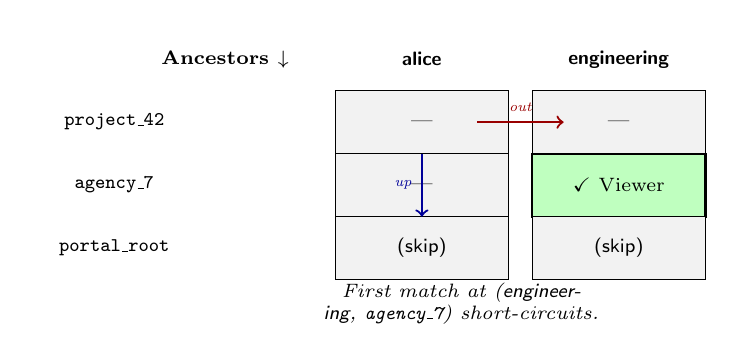
\begin{tikzpicture}[
  cell/.style={minimum width=2.2cm, minimum height=0.8cm, draw, font=\scriptsize, anchor=center},
  header/.style={minimum width=2.2cm, minimum height=0.8cm, font=\scriptsize\bfseries, anchor=center},
  match/.style={cell, fill=green!25, thick},
  miss/.style={cell, fill=gray!10},
]

% Column headers (ancestors - bottom to top)
\node[header] at (0, 3.2) {Ancestors $\downarrow$};
\node[header] at (2.5, 3.2) {\textsf{alice}};
\node[header] at (5.0, 3.2) {\textsf{engineering}};

% Row headers and cells
% Row 1: project_42
\node[header, anchor=east] at (-0.3, 2.4) {\texttt{project\_42}};
\node[miss] at (2.5, 2.4) {---};
\node[miss] at (5.0, 2.4) {---};

% Row 2: agency_7
\node[header, anchor=east] at (-0.3, 1.6) {\texttt{agency\_7}};
\node[miss] at (2.5, 1.6) {---};
\node[match] at (5.0, 1.6) {\checkmark{} Viewer};

% Row 3: portal_root
\node[header, anchor=east] at (-0.3, 0.8) {\texttt{portal\_root}};
\node[miss] at (2.5, 0.8) {\textsf{(skip)}};
\node[miss] at (5.0, 0.8) {\textsf{(skip)}};

% Arrows
\draw[->, thick, blue!60!black] (2.5, 2.0) -- (2.5, 1.2) node[midway, left, font=\tiny\itshape] {up};
\draw[->, thick, red!60!black] (3.2, 2.4) -- (4.3, 2.4) node[midway, above, font=\tiny\itshape] {out};

% Label
\node[font=\scriptsize\itshape, text width=5.5cm, align=center] at (3.0, 0.1) {First match at (\textsf{engineering}, \texttt{agency\_7}) short-circuits.};

\end{tikzpicture}
\caption{Two-dimensional resolution for $\mathit{allowed}(\text{alice}, \textsc{project\_view}, \texttt{project\_42}, \mathit{now})$. The principal set is expanded outward (columns) while the ancestor chain is walked upward (rows). The first matching grant short-circuits evaluation.}
\label{fig:resolution}
\end{figure}

\subsection{Properties}

\begin{property}[Monotonicity of Hierarchy]
If $\mathit{allowed}(p, \mathit{perm}, r, t)$ and $r' \in \mathit{descendants}(r)$, then the same grant provides access at $r'$.
\end{property}
\begin{proof}
If $(p', \mathit{role}, r_{\mathit{anc}}) \in \mathit{active}(t)$ and $r_{\mathit{anc}} \in \mathit{ancestors}(r)$, then since $r' \in \mathit{descendants}(r)$, we have $r \in \mathit{ancestors}(r')$, and by transitivity $r_{\mathit{anc}} \in \mathit{ancestors}(r')$. Therefore the same grant satisfies the access decision for $r'$. \qed
\end{proof}

\begin{property}[Monotonicity of Groups]
Adding $p$ to group $g$ preserves existing access and may grant additional access.
\end{property}
\begin{proof}
Adding $p$ to group $g$ expands $\mathit{resolve}(p)$ to $\mathit{resolve}(p) \cup \{g\}$. Since the access decision uses existential quantification over $\mathit{resolve}(p)$, all previously satisfying assignments remain valid. Any grant held by $g$ additionally becomes effective for $p$. \qed
\end{proof}

\begin{property}[Bounded Evaluation]
For any access decision, evaluation examines at most $|\mathit{resolve}(p)| \times |\mathit{ancestors}(r)| \times G_{\max}$ grant entries, giving $O(M \cdot D \cdot G_{\max})$.
\end{property}

% ===========================================================================
% 4. THE ACCESS EVALUATION ALGORITHM
% ===========================================================================
\section{The Access Evaluation Algorithm}
\label{sec:algorithm}

\subsection{Point Check}

\begin{lstlisting}[style=pseudo]
ALGORITHM PointCheck(p, perm, r, t):
  principals <- resolve(p)
  ancestors <- getAncestors(r)
  FOR EACH r' IN ancestors:
    FOR EACH p' IN principals:
      grants <- getActiveGrants(p', r', t)
      FOR EACH g IN grants:
        IF perm in perms(g.role): RETURN allowed
  RETURN denied
\end{lstlisting}

\subsection{List Filter}

For list filtering, the algorithm is expressed as a SQL predicate:

\begin{lstlisting}[style=pseudo]
ALGORITHM ListFilter(p, perm, query, t):
  principals <- resolve(p)
  principalIds <- join(principals, ',')
  permId <- lookupPermissionId(perm)
  now <- UTC_NOW()
  RETURN query.WHERE(entity =>
    EXISTS(fn_IsResourceAccessible(
      entity.ResourceId, principalIds,
      permId, now)))
\end{lstlisting}

The TVF is evaluated per-row by the database engine, composed with user-defined filters, sorting, and pagination into a single execution plan.

% ===========================================================================
% 5. QUERY-COMPOSABLE ENFORCEMENT VIA TVF
% ===========================================================================
\section{Query-Composable Enforcement via TVF}
\label{sec:tvf}

\subsection{The Table-Valued Function}

The enforcement mechanism is an inline Table-Valued Function (iTVF):

\begin{lstlisting}[style=sql]
CREATE FUNCTION dbo.fn_IsResourceAccessible(
    @ResourceId NVARCHAR(128),
    @PrincipalIds NVARCHAR(MAX),
    @PermissionId NVARCHAR(128),
    @Now DATETIME2
)
RETURNS TABLE
AS
RETURN
(
    WITH ancestors AS (
        SELECT Id, ParentId, 0 AS Depth
        FROM Resources WHERE Id = @ResourceId
        UNION ALL
        SELECT r.Id, r.ParentId, a.Depth + 1
        FROM Resources r
        INNER JOIN ancestors a ON r.Id = a.ParentId
        WHERE a.Depth < 10
    )
    SELECT TOP 1 a.Id
    FROM ancestors a
    INNER JOIN Grants g ON a.Id = g.ResourceId
    INNER JOIN RolePermissions rp
      ON g.RoleId = rp.RoleId
    WHERE g.PrincipalId IN (
        SELECT LTRIM(RTRIM(value))
        FROM STRING_SPLIT(@PrincipalIds, ',')
    )
      AND rp.PermissionId = @PermissionId
      AND (g.EffectiveFrom IS NULL
           OR g.EffectiveFrom <= @Now)
      AND (g.EffectiveTo IS NULL
           OR g.EffectiveTo >= @Now)
)
\end{lstlisting}

The recursive CTE walks UP from the target resource to the root (at most $D$ levels), joining against active grants at each ancestor. \texttt{TOP 1} provides existential semantics---one matching grant suffices. The caller-controlled \texttt{@Now} parameter ensures deterministic evaluation across all rows in a query. As an inline TVF, the optimizer composes its body into the calling query's execution plan, enabling authorization, user filtering, sorting, and pagination in a single statement. We use SQL Server as an exemplar because its optimizer aggressively inlines iTVFs; however, the enforcement requires only recursive CTEs and predicate inlining, both supported by PostgreSQL and other modern engines.

\subsection{Correctness}

\begin{theorem}[Soundness]
If the TVF returns a non-empty result for entity $e$, then $\mathit{allowed}(p, \mathit{perm}, e.\mathit{ResourceId}, \mathit{now}) = \text{true}$.
\end{theorem}
\begin{proof}
The recursive CTE produces exactly $\mathit{ancestors}(e.\mathit{ResourceId})$: the base case selects the resource itself, and each recursive step follows $\mathit{parent}$ pointers until the root. The JOIN against \texttt{Grants} on \texttt{ResourceId} and \texttt{PrincipalId~$\in$~resolve($p$)} implements the existential quantification $\exists\,p' \in \mathit{resolve}(p),\; \exists\,r' \in \mathit{ancestors}(r)$ in Definition~1. The temporal predicates (\texttt{EffectiveFrom~$\leq$~@Now}, \texttt{EffectiveTo~$\geq$~@Now}) correspond to $\mathit{active}(t)$. The JOIN against \texttt{RolePermissions} verifies $\mathit{perm} \in \mathit{perms}(\mathit{role})$. A non-empty result therefore witnesses a satisfying $(p', \mathit{role}, r')$ triple. \qed
\end{proof}

\begin{theorem}[Completeness]
If $\mathit{allowed}(p, \mathit{perm}, e.\mathit{ResourceId}, \mathit{now}) = \text{true}$, the TVF returns a non-empty result, provided $\mathit{depth} \leq 10$.
\end{theorem}
\begin{proof}
The CTE with guard \texttt{Depth~$<$~10} produces all ancestors for resources with depth $\leq 10$. For any satisfying witness $(p', \mathit{role}, r')$ in the formal model, the CTE includes $r'$ (since $r' \in \mathit{ancestors}(r)$), the principal filter includes $p'$ (since $p' \in \mathit{resolve}(p)$), and the temporal and role-permission predicates match by construction. The witness therefore produces a matching row. \qed
\end{proof}

\subsection{Composition into Application Queries}

Because the TVF is an inline function, the query optimizer composes its body into the calling query's execution plan. The application layer resolves the principal's group memberships once per request, then appends the TVF as a predicate alongside application-defined filters, cursor pagination, and sorting:

\begin{lstlisting}[basicstyle=\ttfamily\scriptsize, frame=none, xleftmargin=1em]
FUNCTION AuthorizedList(principal, permission,
                        filters, cursor, k):
  principalIds <- ResolveGroupMemberships(principal)
  query <- FROM table
           WHERE Accessible(row.ResourceId,
                   principalIds, permission)
             AND ApplyFilters(row, filters)
             AND row.SortKey > cursor
           ORDER BY row.SortKey
           LIMIT k
  RETURN Execute(query)  // single DB operation
\end{lstlisting}

Authorization, application filtering, pagination, and sorting compose into a single database operation---one round-trip, zero external calls.

% ===========================================================================
% 6. COMPLEXITY ANALYSIS
% ===========================================================================
\section{Complexity Analysis}
\label{sec:complexity}

\subsection{Per-Row TVF Cost}

For a single entity with resource at depth $d \leq D$:

\begin{enumerate}
\item \textbf{CTE expansion:} $O(D)$ index seeks on \texttt{Resources(Id)}.
\item \textbf{Grant matching:} Joins $D$ ancestors against \texttt{Grants(ResourceId, PrincipalId)} and \texttt{RolePermissions(RoleId, PermissionId)}. With $M = |\mathit{resolve}(p)|$ principals, examines at most $D \cdot M \cdot G_{\max}$ candidates.
\item \textbf{TOP 1 exit:} Short-circuits on first match.
\end{enumerate}

\textbf{Per-row cost:} $O(D \cdot M \cdot G_{\max})$. With $D = 5$, $M = 10$, $G_{\max} = 3$: ${\sim}150$ index lookups.

\subsection{Per-Page Cost Under Pagination}

\begin{theorem}[Per-Page Complexity]
Let $N$ be total entities, $k$ the page size, $D$ the max tree depth, $M = |\mathit{resolve}(p)|$, $G_{\max}$ the max active grants per (principal, resource) pair, and $\sigma \in (0,1]$ the selectivity. Assume: (1) index coverage on Resources, Grants, RolePermissions, and entity ResourceId; (2) cursor pagination on an indexed ordering key; (3) nested loops plan with index seeks. Then:
\begin{itemize}
\item \textbf{Dense ($\sigma \approx 1$):} $O(k \cdot D \cdot M \cdot G_{\max})$, simplified to $O(k \cdot D)$ when $M$ and $G_{\max}$ are bounded constants.
\item \textbf{Sparse ($\sigma \to 0$):} $O(k/\sigma \cdot D \cdot M \cdot G_{\max})$. Degenerate case (no access): $O(N \cdot D \cdot M \cdot G_{\max})$.
\end{itemize}
\end{theorem}
\begin{proof}
With cursor pagination, the engine seeks to the cursor position in $O(\log N)$ and evaluates rows sequentially. Each candidate row incurs a TVF evaluation: the CTE performs $O(D)$ index seeks to walk ancestors, each ancestor is joined against Grants ($M$ principal checks, $G_{\max}$ grants each) and RolePermissions (one seek per grant), yielding $O(D \cdot M \cdot G_{\max})$ per row. \texttt{TOP~1} short-circuits on the first matching grant, so this is an upper bound. To collect $k$ authorized rows with selectivity $\sigma$, the engine examines ${\sim}k/\sigma$ candidates. Total: $O(k/\sigma \cdot D \cdot M \cdot G_{\max})$. When $\sigma \approx 1$, this simplifies to $O(k \cdot D \cdot M \cdot G_{\max})$. Critically, the cursor start position is resolved by index seek, not by scanning prior pages, so cost is independent of page depth and dataset size $N$. \qed
\end{proof}

The per-page cost is \emph{parameterized and predictable}---independent of $N$, linear in $D$.

\subsection{Comparison with Alternatives}

\begin{table}[t]
\centering
\caption{Per-page cost comparison across authorization approaches.}
\label{tab:comparison}
\scriptsize
\begin{tabular}{@{}llll@{}}
\toprule
\textbf{Approach} & \textbf{Per-page} & \textbf{Deps.} & \textbf{Consist.} \\
\midrule
SHRBAC (cursor) & $O(k \cdot D)$ & Local DB & Strong \\
LookupResources + IN & $O(\text{graph}) + O(k)$ & External & Eventual \\
Batch post-filter & $O(k/\sigma \cdot \ell)$ & External & Per-check \\
Partial evaluation & $O(k) + O(\text{comp})$ & Policy eng. & Varies \\
Materialized JOIN & $O(k)$ & Denorm. & Eventual \\
\bottomrule
\end{tabular}
\end{table}

\subsection{Known Considerations}

\texttt{STRING\_SPLIT} produces poor cardinality estimates; table-valued parameters are recommended for $M > 5$. CTE traversal is not short-circuitable; a closure table replaces $O(D)$ recursive expansion with $O(1)$ lookup for deep hierarchies. Plan shape assumes nested loops with index seeks (observed under correct indexing); stale statistics may produce hash joins, mitigated by \texttt{UPDATE STATISTICS}.

% ===========================================================================
% 7. EMPIRICAL EVALUATION
% ===========================================================================
\section{Empirical Evaluation}
\label{sec:empirical}

We evaluate SHRBAC on SQL Server 2022 (Docker, 4 vCPU, 8~GB RAM) across three tiers: (1)~small-scale isolation tests (1K--100K entities) that individually vary each factor, (2)~a production-scale workload at $D{=}5$ with 1.2M resource nodes, and (3)~a deep-hierarchy workload at $D{=}10$ with 1.5M resource nodes.

\subsection{Benchmark Methodology}

\textbf{Measurement protocol.} Each query: 3 warmup runs (discarded), 20 measured runs. Each run opens a fresh connection and records wall-clock elapsed time via \texttt{Stopwatch}. We report median, P95, and IQR. Page size $k = 20$ unless stated otherwise.

\textbf{Query pattern.} All list filtering benchmarks execute the canonical authorized-list query:

\begin{lstlisting}[style=sql]
SELECT TOP (@k) p.Id, p.Name, p.SKU,
       p.Price, p.ResourceId
FROM Products p
WHERE EXISTS (
    SELECT 1 FROM dbo.fn_IsResourceAccessible(
        p.ResourceId, @principalIds,
        'product_view'))
AND p.Id > @cursor
ORDER BY p.Id
\end{lstlisting}

Point checks use the same TVF against a single ResourceId. Query plans verified to use nested loops with index seeks.

\textbf{Hierarchies.} $D{=}5$: root $\to$ 15 chains $\to$ 150 regions $\to$ 15K stores $\to$ 1.2M products = \textbf{1,215,166 resources}. $D{=}10$: root $\to$ 5 divisions $\to$ 25 regions $\to$ 125 districts $\to$ 500 areas $\to$ 2K zones $\to$ 12K stores $\to$ 60K departments $\to$ 240K sections $\to$ 1.2M products = \textbf{1,514,656 resources}. Resources and domain rows are bulk-inserted; \texttt{UPDATE STATISTICS} is run before benchmarks.

\textbf{Isolation tests.} All benchmarks use the same retail SaaS domain model. Isolation tests (Benchmarks 1--7) seed a hierarchy of real domain tables scaled to the target depth: at $D{=}3$, root $\to$ Regions (10) $\to$ Stores (100) $\to$ Products ($N$); at $D{=}5$, root $\to$ Divisions (10) $\to$ Chains (100) $\to$ Regions (1K) $\to$ Stores (10K) $\to$ Products ($N$). Each intermediate level has its own domain table with domain-appropriate columns, and each row maps to a unique resource in the tree. The benchmark query always targets the Products table, ensuring that even small-scale isolation tests exercise the same schema structure and query patterns as the production-scale benchmarks.

\subsection{Isolation Tests (1K--100K)}

Table~\ref{tab:isolation} presents results from controlled single-factor experiments, re-seeded for each configuration to isolate individual factors.

\begin{table}[t]
\centering
\caption{Isolation test results. $k{=}20$ throughout.}
\label{tab:isolation}
\scriptsize
\begin{tabular}{@{}llrr@{}}
\toprule
\textbf{Experiment} & \textbf{Configuration} & \textbf{Med.\ (ms)} & \textbf{P95 (ms)} \\
\midrule
\multirow{5}{*}{$N$ (resource count)} & $N{=}$1K, $D{=}$3 & 3.57 & 4.19 \\
 & $N{=}$5K, $D{=}$3 & 3.51 & 4.58 \\
 & $N{=}$10K, $D{=}$3 & 3.39 & 4.01 \\
 & $N{=}$50K, $D{=}$3 & 3.63 & 4.05 \\
 & $N{=}$100K, $D{=}$3 & 3.32 & 4.07 \\
\addlinespace
\multirow{5}{*}{Depth} & $D{=}$1, $N{=}$10K & 2.45 & 4.90 \\
 & $D{=}$2, $N{=}$10K & 2.94 & 3.96 \\
 & $D{=}$3, $N{=}$10K & 3.17 & 6.16 \\
 & $D{=}$4, $N{=}$10K & 3.55 & 4.43 \\
 & $D{=}$5, $N{=}$10K & 4.21 & 4.79 \\
\addlinespace
\multirow{4}{*}{Principal set ($M$)} & $M{=}$1, $N{=}$10K & 3.47 & 5.53 \\
 & $M{=}$4, $N{=}$10K & 3.14 & 3.75 \\
 & $M{=}$11, $N{=}$10K & 3.45 & 4.81 \\
 & $M{=}$21, $N{=}$10K & 3.32 & 4.09 \\
\addlinespace
\multirow{2}{*}{TVF vs.\ mater.} & TVF EXISTS, $N{=}$100K & 3.42 & 3.97 \\
 & Materialized JOIN, $N{=}$100K & 1.01 & 1.28 \\
\addlinespace
\multirow{2}{*}{Pagination} & Cursor, $N{=}$100K & 3.30 & 4.22 \\
 & Offset COUNT, $N{=}$100K & 2{,}310 & 2{,}473 \\
\bottomrule
\end{tabular}
\end{table}

These isolation results confirm core predictions: $N$-independence across 1K--100K (3.32--3.63ms at $D{=}3$), monotonic depth scaling from 2.45ms at $D{=}1$ to 4.21ms at $D{=}5$ consistent with $O(k \cdot D)$, negligible principal set size effect (3.14--3.47ms across $M{=}1$--$21$), and constant cursor pagination cost independent of dataset size. The question is whether these properties hold at production resource scale.

\subsection{Production-Scale at $D{=}5$ (1.2M Resources)}

We constructed a retail SaaS hierarchy: root $\to$ 15 chains $\to$ 150 regions $\to$ 15K stores $\to$ 1.2M products, yielding \textbf{1,215,166 resource nodes} at $D{=}5$. Principals range from company administrators (all 1.2M products accessible) to store managers (${\sim}$80 products).

Table~\ref{tab:production} presents results across three dimensions.

\begin{table}[t]
\centering
\caption{Production-scale results at 1.2M resources, $D{=}5$.}
\label{tab:production}
\scriptsize
\begin{tabular}{@{}llrr@{}}
\toprule
\textbf{Sub-experiment} & \textbf{Configuration} & \textbf{Med.\ (ms)} & \textbf{P95 (ms)} \\
\midrule
\multirow{4}{*}{Page size ($k$)} & $k{=}10$ & 2.28 & 7.59 \\
 & $k{=}20$ & 3.47 & 4.55 \\
 & $k{=}50$ & 6.89 & 8.65 \\
 & $k{=}100$ & 13.71 & 20.25 \\
\addlinespace
\multirow{4}{*}{Scope level} & Company admin (1.2M) & 3.47 & 4.55 \\
 & Chain manager (${\sim}$80K) & 3.20 & 3.95 \\
 & Region manager (${\sim}$8K) & 3.11 & 6.34 \\
 & Store manager (${\sim}$80) & 2.02 & 2.57 \\
\addlinespace
\multirow{3}{*}{Deep cursor} & Page 1 & 3.08 & 4.04 \\
 & ${\sim}$Page 50 & 3.25 & 3.63 \\
 & ${\sim}$Page 500 & 3.48 & 4.28 \\
\bottomrule
\end{tabular}
\end{table}

\textbf{Page size} scales linearly: the ratio $13.71/2.28 = 6.01\times$ for a $10\times$ increase in $k$ confirms $O(k)$. Per-row cost at $D{=}5$: ${\sim}$0.14ms, corresponding to ${\sim}$0.034ms per CTE hop.

\textbf{Scope level}: despite a $15{,}000\times$ difference in accessible product count, latency varies minimally---store-level grants fastest in median because CTE short-circuits.

\textbf{Cursor depth} is flat: page 500 at 3.48ms is indistinguishable from page~1 at 3.08ms.

\subsection{Deep Hierarchy at $D{=}10$ (1.5M Resources)}

To test whether $O(k \cdot D)$ scaling holds at deeper hierarchies, we constructed a 10-level tree yielding \textbf{1,514,656 resource nodes}. Table~\ref{tab:d10} compares identical queries across both tree depths.

\begin{table}[t]
\centering
\caption{Page size comparison: $D{=}5$ vs.\ $D{=}10$.}
\label{tab:d10}
\scriptsize
\begin{tabular}{@{}lrrr@{}}
\toprule
$k$ & \textbf{$D{=}5$ (ms)} & \textbf{$D{=}10$ (ms)} & \textbf{Ratio} \\
\midrule
10 & 2.28 & 3.44 & 1.51$\times$ \\
20 & 3.47 & 5.69 & 1.64$\times$ \\
50 & 6.89 & 11.80 & 1.71$\times$ \\
100 & 13.71 & 22.01 & 1.61$\times$ \\
\bottomrule
\end{tabular}
\end{table}

The $D{=}10$/$D{=}5$ ratio ranges from $1.51\times$ to $1.71\times$. Per-row cost at $D{=}10$: ${\sim}$0.22ms, or ${\sim}$0.024ms per CTE hop. The per-hop cost difference (0.034ms at $D{=}5$ vs 0.024ms at $D{=}10$) suggests fixed per-page overhead is proportionally larger at $D{=}5$; at larger $k$ the costs converge.

Scope-level and cursor-depth results at $D{=}10$ mirror $D{=}5$: scope varies minimally (3.06--5.54ms), and cursor depth is flat (5.11--5.38ms across pages 1--500).

\subsection{Point Access Checks}

While SHRBAC's primary contribution is list filtering, the TVF also serves as a point check. Table~\ref{tab:pointcheck} measures point check latency at both $D{=}5$ (1.2M resources) and $D{=}10$ (1.5M resources).

\begin{table}[t]
\centering
\caption{Point access check latency. $D{=}5$: 1.2M resources; $D{=}10$: 1.5M resources.}
\label{tab:pointcheck}
\scriptsize
\begin{tabular}{@{}llrr@{}}
\toprule
\textbf{Depth} & \textbf{Level} & \textbf{$D{=}5$ (ms)} & \textbf{$D{=}10$ (ms)} \\
\midrule
0 & Root & 0.86 & 0.89 \\
1 & Chain / Division & 0.97 & 0.95 \\
2 & Region & 1.06 & 1.27 \\
3 & Store / District & 1.04 & 0.99 \\
4 & Product / Area & 1.31 & 1.09 \\
5--9 & (D=10 only) & --- & 1.13--1.46 \\
\bottomrule
\end{tabular}
\end{table}

Even at depth~9 with 1.5M resource nodes, all point checks complete in \textbf{under 1.5ms median}. Grant set size (1--20 active grants) produces 1.19--1.38ms---flat. Principal set size ($M{=}1$--$21$) produces 0.98--1.28ms---near-constant. The CTE examines only the target resource's ancestor chain (${\leq}D$ nodes), not the grant table at large.

\subsection{Factor Analysis}

The multi-dimensional benchmarks at 1.2M resources ($D{=}5$) and 1.5M resources ($D{=}10$) enable a comprehensive factor analysis (Table~\ref{tab:factors}).

\begin{table*}[t]
\centering
\caption{Factor sensitivity analysis at production scale. Results from $D{=}5$ (1.2M resources) and $D{=}10$ (1.5M resources).}
\label{tab:factors}
\scriptsize
\begin{tabular}{@{}lllllc@{}}
\toprule
\textbf{Factor} & \textbf{Range} & \textbf{List filter effect} & \textbf{Point check effect} & \textbf{Predicted} & \textbf{Confirmed?} \\
\midrule
$N$ (resource count) & 1K--1.5M & None (3.39ms $\to$ 3.47ms*) & N/A (CTE-local) & $O(1)$ & \checkmark \\
$k$ (page size) & 10--100 & Linear (2.28--13.71ms $D{=}5$; 3.44--22.01ms $D{=}10$) & N/A & $O(k)$ & \checkmark \\
$D$ (tree depth) & 1--10 & Linear (2.45 $\to$ 4.21 $\to$ 5.69ms) & Sub-1.5ms both & $O(D)$ & \checkmark \\
Per-hop cost & $D{=}5$ vs $D{=}10$ & 0.034ms $D{=}5$, 0.024ms $D{=}10$ & --- & $O(1)$ & \checkmark \\
$M$ (principals) & 1--11 & Negligible (3.32--3.44ms $D{=}5$; 5.42--5.85ms $D{=}10$) & None (0.98--1.28ms) & $O(M)$ & Negligible \\
$G$ (grant density) & 1--10 & None (3.23--3.40ms $D{=}5$; 5.00--5.80ms $D{=}10$) & None (1.19--1.38ms) & $O(G_{\max})$ & Refuted \\
Cursor depth & Page 1--500 & None (3.08--3.48ms $D{=}5$; 5.11--5.38ms $D{=}10$) & N/A & $O(1)$ & \checkmark \\
\bottomrule
\end{tabular}
\end{table*}

\noindent *The 10K$\to$1.2M increase (3.39$\to$3.47ms) compares $D{=}3$ isolation vs $D{=}5$ production; the difference is attributable to depth, not resource count.

Table~\ref{tab:dimensional} presents the dimensional analysis at $D{=}5$.

\begin{table}[t]
\centering
\caption{Dimensional analysis at 1.2M resources, $D{=}5$, $k{=}20$.}
\label{tab:dimensional}
\scriptsize
\begin{tabular}{@{}llr@{}}
\toprule
\textbf{Dimension} & \textbf{Configuration} & \textbf{Med.\ (ms)} \\
\midrule
\multirow{4}{*}{Principal set (list)} & $M{=}1$ & 3.36 \\
 & $M{=}3$ & 3.32 \\
 & $M{=}6$ & 3.36 \\
 & $M{=}11$ & 3.44 \\
\addlinespace
\multirow{4}{*}{Grant density} & 1 chain (${\sim}$80K accessible) & 3.31 \\
 & 3 chains (${\sim}$240K) & 3.23 \\
 & 5 chains (${\sim}$400K) & 3.41 \\
 & 10 chains (${\sim}$800K) & 3.40 \\
\addlinespace
\multirow{4}{*}{Grant depth} & Chain grant (inherit all) & 3.12 \\
 & 100 store grants & 4.27 \\
 & 10 store grants & 2.50 \\
 & 1 store grant & 2.28 \\
\bottomrule
\end{tabular}
\end{table}

\subsection{Analysis}

% ---- FIGURE: N-independence across three orders of magnitude ----
\begin{figure}[t]
\centering
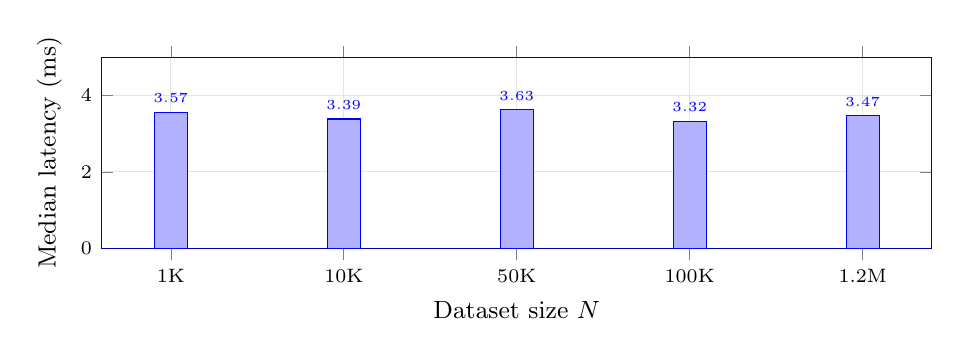
\begin{tikzpicture}
\begin{axis}[
    width=\columnwidth,
    height=4.0cm,
    xlabel={Dataset size $N$},
    ylabel={Median latency (ms)},
    symbolic x coords={1K,10K,50K,100K,1.2M},
    xtick=data,
    ymin=0, ymax=5,
    ybar,
    bar width=12pt,
    nodes near coords,
    nodes near coords style={font=\tiny},
    every node near coord/.append style={above},
    grid=major,
    grid style={gray!20},
    every axis label/.style={font=\small},
    every tick label/.style={font=\scriptsize},
    fill=blue!50,
    draw=blue!70!black,
]
\addplot coordinates {(1K, 3.57) (10K, 3.39) (50K, 3.63) (100K, 3.32) (1.2M, 3.47)};
\end{axis}
\end{tikzpicture}
\caption{Per-page median latency ($k{=}20$, cursor) across three orders of magnitude. Latency remains flat at ${\sim}$3.3--3.6ms. The small increase at 1.2M is attributable to depth ($D{=}5$ vs $D{=}3$), not resource count.}
\label{fig:scaling}
\end{figure}

\textbf{$N$-independence extends to 1.5M resources (Fig.~\ref{fig:scaling}).} With 1,215,166 unique resource nodes at $D{=}5$, list filtering median is 3.47ms ($k{=}20$)---compared to 3.39ms at $N{=}$10K with $D{=}3$ in isolation tests. The small increase is attributable to depth ($D{=}5$ vs $D{=}3$), not resource count. At $D{=}10$ with 1,514,656 resources, per-page cost is 5.69ms---again a depth effect.

\textbf{Per-hop cost.} At $D{=}5$, per-row cost is ${\sim}$0.14ms (4 CTE hops $\times$ 0.034ms/hop). At $D{=}10$, per-row cost is ${\sim}$0.22ms (9 CTE hops $\times$ 0.024ms/hop). The per-hop cost converges at higher page sizes as fixed per-page overhead diminishes, giving $O(k \cdot D)$ a concrete, measurable constant.

\textbf{Grant density remains irrelevant.} At $D{=}5$: 3.31 vs.\ 3.40ms---a 0.09ms difference for a $10\times$ increase. At $D{=}10$: 5.00 vs.\ 5.76ms. The TVF evaluates each row via its ancestor chain; the breadth of authority does not affect per-row cost.

% ---- FIGURE: Leaf grants vs inherited grants ----
\begin{figure}[t]
\centering
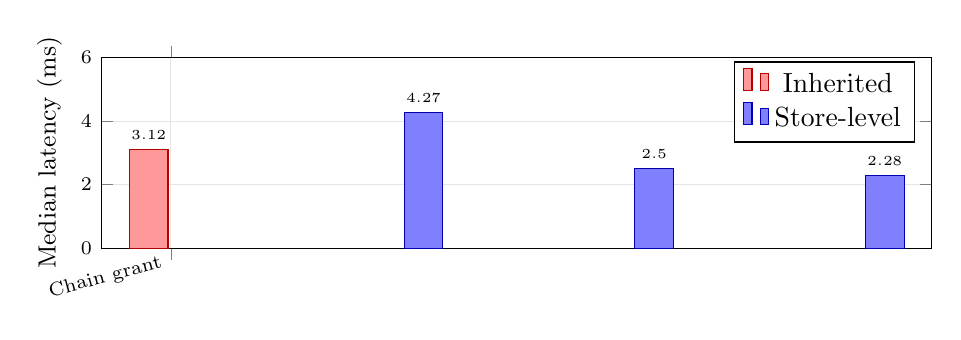
\begin{tikzpicture}
\begin{axis}[
    width=\columnwidth,
    height=4.0cm,
    ylabel={Median latency (ms)},
    symbolic x coords={Chain grant,{100 stores},{10 stores},{1 store}},
    xtick=data,
    ymin=0, ymax=6,
    ybar,
    bar width=14pt,
    nodes near coords,
    nodes near coords style={font=\tiny},
    every node near coord/.append style={above},
    grid=major,
    grid style={gray!20},
    every axis label/.style={font=\small},
    every tick label/.style={font=\scriptsize},
    x tick label style={rotate=15, anchor=east},
]
\addplot[fill=red!40, draw=red!70!black] coordinates {(Chain grant, 3.12)};
\addplot[fill=blue!50, draw=blue!70!black] coordinates {({100 stores}, 4.27) ({10 stores}, 2.50) ({1 store}, 2.28)};
\legend{Inherited, Store-level}
\end{axis}
\end{tikzpicture}
\caption{Store-level grants outperform inherited grants at 1.2M resources. A single store grant (2.28ms) is 27\% faster than a chain-level grant (3.12ms). The CTE walks UP from the product; grants closer to the leaf short-circuit sooner.}
\label{fig:leafgrants}
\end{figure}

\textbf{Least-privilege grants outperform inherited grants (Fig.~\ref{fig:leafgrants}).} A chain-level grant (3.12ms) is 37\% slower than a single store grant (2.28ms). The CTE walks UP from the product toward the root; a store-level grant matches at the first ancestor hop, while a chain-level grant requires 3--4 hops. This validates the short-circuit property and reveals that least-privilege grants are not only more secure---they are faster.

\textbf{Principal set size is negligible.} $M{=}1$ vs $M{=}11$ produces 3.36 vs.\ 3.44ms. At $D{=}10$: 5.63 vs.\ 5.85ms. \texttt{STRING\_SPLIT} overhead is negligible at practical principal counts.

\textbf{Point checks are sub-1.5ms even at $D{=}10$.} At depth~9 (the deepest leaf), point checks complete in 1.32ms median. Grant set size (1--20) and principal set size ($M{=}1$--$21$) have no measurable impact.

\textbf{Page size scales linearly.} $k{=}10 \to 100$ yields 2.28 $\to$ 13.71ms ($6.01\times$ for $10\times$). At 1.5M resources ($D{=}10$): 3.44 $\to$ 22.01ms ($6.40\times$ for $10\times$). Both closely track $O(k)$.

\textbf{Cursor vs.\ offset pagination (Fig.~\ref{fig:pagination}).} Offset COUNT costs grow linearly: 231ms ($N{=}$10K) $\to$ 1{,}114ms ($N{=}$50K) $\to$ 2{,}310ms ($N{=}$100K). Cursor pagination remains at ${\sim}$3.3ms. At $N{=}$100K, cursor is $700\times$ faster.

% ---- FIGURE: Cursor vs Offset pagination ----
\begin{figure}[t]
\centering
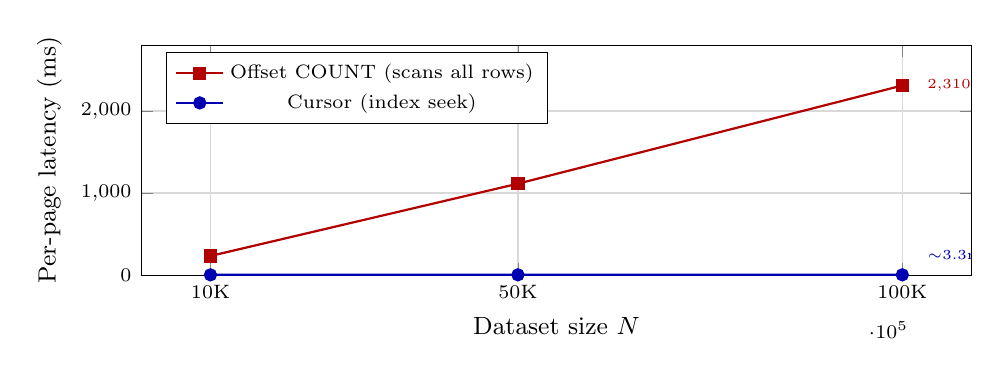
\begin{tikzpicture}
\begin{axis}[
    width=\columnwidth,
    height=4.5cm,
    xlabel={Dataset size $N$},
    ylabel={Per-page latency (ms)},
    xtick={10000,50000,100000},
    xticklabels={10K,50K,100K},
    ymin=0, ymax=2800,
    legend style={at={(0.03,0.97)}, anchor=north west, font=\scriptsize},
    grid=major,
    grid style={gray!30},
    every axis label/.style={font=\small},
    every tick label/.style={font=\scriptsize},
]

% Offset line
\addplot[
    color=red!70!black,
    mark=square*,
    thick,
    mark size=2pt,
] coordinates {
    (10000, 233)
    (50000, 1114)
    (100000, 2310)
};
\addlegendentry{Offset COUNT (scans all rows)}

% Cursor line
\addplot[
    color=blue!70!black,
    mark=*,
    thick,
    mark size=2pt,
] coordinates {
    (10000, 3.20)
    (50000, 3.45)
    (100000, 3.30)
};
\addlegendentry{Cursor (index seek)}

% Annotations
\node[font=\tiny, anchor=west, text=red!70!black] at (axis cs:102000,2310) {2{,}310ms};
\node[font=\tiny, anchor=west, text=blue!70!black] at (axis cs:102000,250) {$\sim$3.3ms};

\end{axis}
\end{tikzpicture}
\caption{Offset COUNT per-page cost grows linearly with $N$: 231ms ($N{=}$10K) $\to$ 1{,}114ms ($N{=}$50K) $\to$ 2{,}310ms ($N{=}$100K). Cursor pagination maintains ${\sim}$3.3ms. At $N{=}$100K, cursor is $700\times$ faster.}
\label{fig:pagination}
\end{figure}

\textbf{TVF vs.\ materialized.} The materialized approach is ${\sim}$3.4$\times$ faster per-page (1.01ms vs.\ 3.42ms at $N{=}$100K) but requires denormalization infrastructure. Both are $N$-independent under cursor pagination. SHRBAC's TVF provides strong consistency with zero infrastructure overhead.

% ===========================================================================
% 8. DISCUSSION
% ===========================================================================
\section{Discussion}
\label{sec:discussion}

The theoretical analysis in Sections~\ref{sec:model}--\ref{sec:complexity} established that SHRBAC's per-page enforcement cost is $O(k \cdot D)$, and the empirical results in Section~\ref{sec:empirical} confirmed this bound across three orders of magnitude. This section examines the design trade-offs that make these guarantees possible, positions SHRBAC relative to alternative authorization models, and discusses implications for agentic systems.

\subsection{Constraints as Architectural Choice}

SHRBAC's performance guarantees are a direct consequence of four structural constraints. Each constraint eliminates a source of unbounded computation in the enforcement path:

\begin{theorem}[Constraint-Composability Tradeoff]
SHRBAC intentionally disallows: (C1)~DAG-structured resources---resources form a tree, not a DAG; (C2)~recursive group membership---groups cannot contain groups; (C3)~role hierarchies---roles are flat; (C4)~arbitrary attribute predicates---only role + resource-scope + time are evaluated. In return: (G1)~CTE traversal is bounded at $O(D)$; (G2)~principal resolution is a single join producing a fixed set; (G3)~the TVF body is fixed at schema design time---no runtime policy compilation; (G4)~enforcement is a standard SQL \texttt{EXISTS} subquery composable with arbitrary \texttt{WHERE}, \texttt{ORDER BY}, and pagination.
\end{theorem}

Each constraint enables its corresponding guarantee. Relaxing (C1) to allow DAGs replaces a unique bounded ancestor chain with potentially unbounded multiple ancestor paths, eliminating deterministic $O(D)$ traversal and breaking~(G1). Relaxing~(C2) to allow nested groups turns principal resolution into a recursive traversal, breaking~(G2). Relaxing~(C3) to allow role inheritance requires transitive closure at evaluation time, breaking~(G3). Relaxing~(C4) to allow arbitrary predicates requires runtime policy compilation, breaking~(G4).

Crucially, these constraints are not artificial restrictions imposed to simplify the model---they codify the \emph{de facto} structure of most multi-tenant B2B SaaS systems. Resource containment naturally forms a tree rooted at a tenant boundary (organization $\to$ departments $\to$ projects $\to$ artifacts). Groups are typically flat membership lists. Roles enumerate permissions rather than inheriting from other roles. SHRBAC formalizes this common but undocumented pattern and demonstrates that when the dominant structural assumptions are embraced explicitly, strong composability and performance guarantees follow.

\subsection{Relationship to ABAC and ReBAC}

SHRBAC evaluates two attributes---role and resource-scope---making it a two-attribute constrained ABAC system~\cite{abac-nist}. The resource tree can be viewed as a constrained ReBAC graph where all relationships are \texttt{parent\_of} typed and the graph is a tree. The tree constraint (bounded depth, deterministic ancestor chains) is what makes TVF enforcement tractable. For applications requiring arbitrary relationship graphs, ReBAC/Zanzibar is more appropriate; for organizational hierarchies, SHRBAC's constraint matches the domain and provides predictable performance.

\subsection{SHRBAC for Agentic Systems}

SHRBAC's polymorphic principal model naturally accommodates autonomous AI agents. An agent is a principal with $\tau(p) = \text{agent}$ that participates in the same grant relation as human users, with three properties critical for agent governance:

\textbf{Least-privilege delegation.} SHRBAC's grant triple (principal, role, resource) with temporal bounds directly enforces least-privilege delegation: an agent receives only the role it needs, at only the resource subtree it operates on, for only the duration of its task. A 15-minute grant at a specific project subtree is expressible directly, without special-case logic.

\textbf{Predictable query cost.} Agents that enumerate resources in loops amplify per-query costs. The TVF's $O(k \cdot D)$ per-page bound ensures that agent-driven queries have predictable, bounded database impact regardless of how many resources exist---preventing runaway load from autonomous operations.

\textbf{Auditability.} Every agent action traces to a specific (agent, role, resource) grant with temporal bounds. When an agent's authority expires ($\mathit{EffectiveTo} < \mathit{now}$), access ceases immediately without requiring token revocation infrastructure.

\subsection{Scope and Limitations}

\begin{itemize}
\item \textbf{Tree constraint (C1):} DAG resources (matrix management, multi-parent projects) are not supported. ReBAC is more appropriate for these domains.
\item \textbf{Non-recursive groups (C2):} Deeply nested group structures require extending $\mathit{resolve}(p)$ with CTE traversal.
\item \textbf{Flat roles (C3):} Role definitions must explicitly enumerate permissions rather than inheriting.
\item \textbf{No arbitrary attributes (C4):} IP-based, device-type, or other dynamic attribute conditions are not expressible.
\item \textbf{Database engine:} Portability requirements discussed in \S\ref{sec:tvf}. PostgreSQL and MySQL 8.0+ support the necessary primitives (recursive CTEs, predicate inlining).
\end{itemize}

% ===========================================================================
% 9. CONCLUSION
% ===========================================================================
\section{Conclusion}
\label{sec:conclusion}

We presented SHRBAC, a formal authorization model whose structural constraints guarantee that per-page enforcement cost is $O(k \cdot D)$---linear in page size and tree depth, independent of total resource count and policy set size. The model sits at the intersection of hierarchical RBAC (ROBAC/RRBAC), polymorphic principal resolution, and Stonebraker's query modification.

Empirical evaluation at 1.2M resources ($D{=}5$) and 1.5M resources ($D{=}10$) confirms the predicted complexity: per-page latency is $N$-independent across three orders of magnitude, scales linearly with $k$ and $D$, and is unaffected by grant density or cursor depth. The per-CTE-hop cost is constant across both tree depths, giving $O(k \cdot D)$ a measurable constant. A notable finding is that least-privilege grants are not only more secure but faster---the upward tree walk short-circuits sooner at narrower scopes.

As autonomous agents become principals in enterprise systems, the need for scoped, auditable, time-bounded authorization with efficient list filtering will intensify. SHRBAC's grant model---where an agent receives exactly the authority it needs, at the scope it needs, for the duration it needs---provides a foundation for database-native agent governance without requiring external authorization infrastructure.

% ===========================================================================
% ACKNOWLEDGMENTS
% ===========================================================================
\section*{Acknowledgments}
{[Removed for double-blind review.]}

\smallskip\noindent\textit{AI Disclosure:} In accordance with IEEE policy, the authors disclose that AI tools (Claude, Anthropic) were used to assist with manuscript preparation and editing. All technical content, formal definitions, proofs, implementation, and experimental design are the work of the authors.

% ===========================================================================
% REFERENCES
% ===========================================================================
\balance
\begin{thebibliography}{20}

\bibitem{zanzibar}
R.~Pang et~al., ``Zanzibar: Google's Consistent, Global Authorization System,'' in \emph{Proc. USENIX ATC}, 2019.

\bibitem{saltzer}
J.~H. Saltzer and M.~D. Schroeder, ``The Protection of Information in Computer Systems,'' \emph{Proc. IEEE}, vol.~63, no.~9, pp.~1278--1308, 1975.

\bibitem{robac}
Z.~Zhang, X.~Zhang, and R.~Sandhu, ``ROBAC: Scalable Role and Organization Based Access Control Models,'' in \emph{Proc. CollaborateCom}, 2006.

\bibitem{stonebraker}
M.~Stonebraker and E.~Wong, ``Access Control in a Relational Data Base Management System by Query Modification,'' in \emph{Proc. ACM National Conf.}, 1974, pp.~180--187.

\bibitem{rbac96}
R.~Sandhu, E.~J. Coyne, H.~L. Feinstein, and C.~E. Youman, ``Role-Based Access Control Models,'' \emph{IEEE Computer}, vol.~29, no.~2, pp.~38--47, 1996.

\bibitem{nist-rbac}
D.~F. Ferraiolo et~al., ``Proposed NIST Standard for Role-Based Access Control,'' \emph{ACM TISSEC}, vol.~4, no.~3, pp.~224--274, 2001.

\bibitem{rrbac}
N.~Solanki et~al., ``Resource and Role Hierarchy Based Access Control for Resourceful Systems,'' in \emph{Proc. IEEE COMPSAC}, pp.~396--401, 2018.

\bibitem{orbac}
A.~Abou El~Kalam et~al., ``Organization Based Access Control,'' in \emph{Proc. IEEE POLICY}, 2003.

\bibitem{rizvi}
S.~Rizvi, A.~Mendelzon, S.~Sudarshan, and P.~Roy, ``Extending Query Rewriting Techniques for Fine-Grained Access Control,'' in \emph{Proc. ACM SIGMOD}, pp.~551--562, 2004.

\bibitem{sieve}
P.~Pappachan, R.~Yus, S.~Mehrotra, and J.-C. Freytag, ``Sieve: A Middleware Approach to Scalable Access Control for Database Management Systems,'' \emph{PVLDB}, vol.~13, no.~12, 2020.

\bibitem{fong}
P.~W.~L. Fong, ``Relationship-Based Access Control: Protection Model and Policy Language,'' in \emph{Proc. CODASPY}, pp.~191--202, 2011.

\bibitem{authzed}
AuthZed, ``Protecting a List Endpoint,'' SpiceDB Documentation. [Online].

\bibitem{oso}
Oso, ``List Filtering,'' Oso Documentation. [Online].

\bibitem{cerbos}
Cerbos, ``Filtering Data Using Authorization Logic,'' Cerbos Blog. [Online].

\bibitem{abac-nist}
V.~C. Hu et~al., ``Guide to Attribute Based Access Control (ABAC) Definition and Considerations,'' \emph{NIST SP 800-162}, 2014.

\bibitem{azure-rbac}
Microsoft, ``What is Azure role-based access control (Azure RBAC)?'' Microsoft Learn. [Online].

\bibitem{trbac}
E.~Bertino, P.~Bonatti, and E.~Ferrari, ``TRBAC: A Temporal Role-Based Access Control Model,'' \emph{ACM TISSEC}, vol.~4, no.~3, 2001.

\bibitem{arbac}
R.~Sandhu, V.~Bhamidipati, and Q.~Munawer, ``The ARBAC97 Model for Role-Based Administration of Roles,'' \emph{ACM TISSEC}, vol.~2, no.~1, pp.~105--135, 1999.

\bibitem{kuhn}
D.~R. Kuhn, E.~J. Coyne, and T.~R. Weil, ``Adding Attributes to Role-Based Access Control,'' \emph{IEEE Computer}, vol.~43, no.~6, pp.~79--81, 2010.

\bibitem{rls}
Microsoft, ``Row-Level Security,'' SQL Server Documentation. [Online].

\end{thebibliography}

\end{document}
